\title{Final for Calculus-Based Physics: Electricity and Magnetism}
\author{Dr. Jordan Hanson - Whittier College Dept. of Physics and Astronomy}
\date{\today}
\documentclass[10pt]{article}
\usepackage[a4paper, total={18cm, 27cm}]{geometry}
\usepackage{outlines}
\usepackage{graphicx}
\usepackage{amsmath}
\begin{document}
\maketitle

\section{Equations and constants}

\begin{enumerate}
\item Volume of a sphere: $V_s = \frac{4}{3}\pi r^3$.
\item Density, mass and volume: $m = \rho V$.
\item Charge density, charge and volume: $Q = \rho V$.
\item Coulomb force: $\vec{F}_C = k \frac{q_1 q_2}{r^2}\hat{r}$.
\item Definition of electric field: $\vec{F}_C = q\vec{E}$.
\item Definition of electric flux: $\phi_E = \vec{E} \cdot \vec{A}$.
\item Gauss' Law: $\phi_E = q_{enc}/\epsilon_0$. (Assumes field is uniform over the surface).
\item Voltage and electric field, one dimension, uniform field: $|E| = - \frac{\Delta V}{\Delta x}$.
\item Voltage and electric field, general case: $\vec{E} = -\nabla V$.
\item Ohm's Law: $V = IR$.
\item Electrical power: $P = IV = I^2 R = V^2/R$.
\item Magnetic dipole moment: $\vec{\mu} = I \vec{A}$, where $\vec{A}$ is the area vector.
\item Torque on a magnetic dipole: $\tau = \vec{\mu} \times \vec{B}$.
\item Definition of magnetic flux: $\phi_m = \vec{B} \cdot \vec{A}$.  The units are T m$^2$, which is called a Weber, or Wb.
\item Faraday's Law: $emf = -N \frac{d \phi}{d t}$
\item Faraday's Law using \textbf{Inductance}, M: $emf = -M \frac{dI}{dt}$.
\item Typically, we refer to \textit{mutual inductance} between two objects as $M$, and \textit{self inductance} as $L$.
\item Inductance of a solenoid: $L = \mu_0 n^2 V$
\item Magnetic permeability: $\mu_0 = 4\pi \times 10^{-7}$ T m A$^{-1}$
\item Units of inductance: V s A$^{-1}$, which is called a Henry, or H.
\item Coulomb constant: $k = 8.9876 \times 10^{9}$ N m$^2$ C$^{-2}$.
\item Fundamental charge: $q_e = 1.602 \times 10^{-19}$ C.
\end{enumerate}

\clearpage

\section{Exercises}

\begin{enumerate}
\item \textbf{Chapters 5-6: Electrostatics and Gauss' Law}
\begin{enumerate}
\item Two charges 3 $\mu$C and 12 $\mu$C are fixed 1 m apart, with the second one to the right. Find the magnitude and direction of the net force on a -2 nC charge when placed at the following locations: (a) halfway between the two (b) half a meter to the left of the left charge. \\ \\
a) 0.6 mN to the right.  b) 0.312 mN to the right. \\
\item Using Gauss' law, prove that the electric field a distance $r$ from an infinite line of charge with charge per unit length $\lambda$ is
\begin{equation}
\vec{E} = \frac{\lambda}{2\pi\epsilon_0 r} \hat{r}
\end{equation} \\ \\
Let $l$ be a segment of the line of charge, with total charge $q = \lambda l$. Applying Gauss' law yields:
\begin{align}
\phi_E &= \vec{E} \cdot \vec{A} = \frac{q_{enc}}{\epsilon_0} \\
q_{enc} &= \lambda l \\
\vec{E} \cdot \vec{A} &= EA \\
EA &= \frac{\lambda l}{\epsilon_0} \\
A &= 2\pi r l \\
E(2\pi r l) &= \frac{\lambda l}{\epsilon_0} \\
\vec{E} &= \frac{\lambda}{2\pi\epsilon_0 r} \hat{r}
\end{align}
The direction is given by symmetry (outward from the wire).
\end{enumerate}
\item \textbf{Chapters 7-8: Voltage and Capacitance}
\begin{enumerate}
\item The voltage across a capacitor is 100 mV, and the distance between the two charged surfaces is 1 mm.  What is the electric field in the capacitor? \\ \\
When the electric field is uniform, the field is given by the voltage divided by the distance: $E = \Delta V / \Delta x = 0.1/10^{-3}$ V/m, or 100 V/m. \\
\item An electric potential is defined by $V(x,y,z) = a x + b \sin(ky)$, with $a = 2.0$ V m$^{-2}$, $b = 1.0$ V m$^{-1}$, and $\omega = 10\pi$ rad m$^{-1}$.  What is the corresponding electric field at $P = (-1,1)$? \\ \\
The negative gradient gives you the electric field:
\begin{align}
\vec{E} = -\nabla V &= -\frac{\partial}{\partial x} (ax)\hat{x} - \frac{\partial}{\partial y} b\sin(ky)\hat{y} \\
\vec{E} &= -a\hat{x}-kb \cos(ky)\hat{y}
\end{align}
\end{enumerate}
\item \textbf{Chapters 9-10: Current, Resistance, and DC Circuits}
\begin{enumerate}
\item Two resistors are connected in series.  One has 1000$\Omega$ resistance, and the other has 500$\Omega$ resistance.  If the resistors are connected in series to a 1.5 V battery, (a) what current will flow? (b) Draw a graph of $I$ vs. $V$ in this system, as if $V$ could vary but the total resistance were fixed.  Label the axes of the graph and indicate the slope. \\ \\
The total resistance is 1500$\Omega$, because the resistors are in series.  Using Ohm's law, we have 1.5V/1500$\Omega$ = 1.0 mA.  The graph is a linear graph, and if we place Volts on the y-axis, and current on the x-axis, the slope will be 1500.  However, if we put current on the y-axis and volts on the x-axis, the slope will be 1/1500. \\
\item How much energy in kiloWatt hours does a $10\Omega$ light consume if it draws 1.0 Amp of current for 6 hours? \\ \\
The relevant equation is $P=IV = I^2 R$.  We have the current and the resistance, so this is a $1.0^2 \times 10.0 = 10.0$ W light bulb.  Thus, a 10W light running for 6 hours consumes 60 W hours of energy, or 0.06 kW hours.  Remember that energy $U = P \Delta t$, so a ``Watt hour'' or ``kW hour'' is an energy, not a power. \\
\item Two AA batteries are connected \textit{in parallel} with a load resistor $R$, as shown in Fig. \ref{fig:batt1} (left).  The two internal resistances are $r_1$ and $r_2$, and the two emf's are $\mathcal{E}_1$ and $\mathcal{E}_2$. Assume $r_1 = r_2$ and $\mathcal{E}_1 = \mathcal{E}_2$.  (a) Using the junction rule once, and the loop rule twice, solve for the current through the load resistor algebraically. (b) If  $\mathcal{E}_1 = \mathcal{E}_2 = 1.5$ V, $r_1 = r_2 = 0.1 \Omega$, and $R = 100\Omega$, what is the current through $R$? \\ \vspace{4cm}
\begin{figure}
\centering
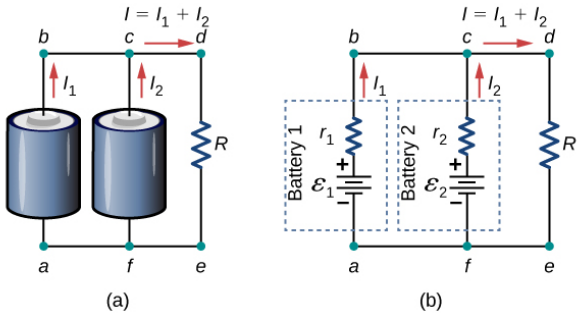
\includegraphics[width=0.4\textwidth]{batt1.png}
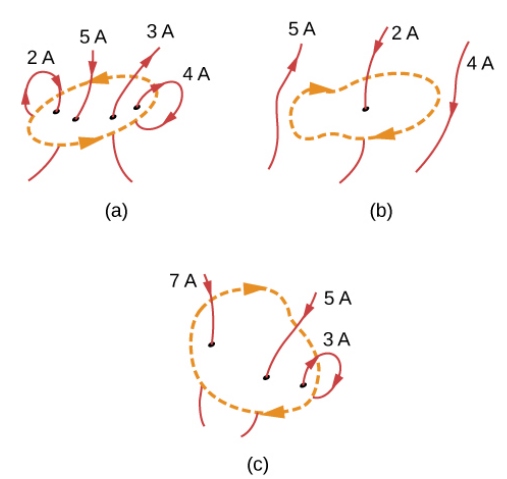
\includegraphics[width=0.3\textwidth]{amplaw.png}
\caption{\label{fig:batt1} (Left) Two batteries (a) connected in parallel with internal resistances can be modelled by a circuit (b). (Right) Three configurations of currents and loops.}
\end{figure}
\end{enumerate}
\item \textbf{Chapters 11-12: Magnetic fields and Sources of Magnetic Fields}
\begin{enumerate}
\item A circular loop of wire of area $10^{-2}$ m$^{2}$ carries a current of 20.0 A.  At a particular instant, the loop lies in the $xy$-plane and is subjected to a magnetic field $\vec{B} = \left( 3.0 \hat{i} + 6.0 \hat{j} + 3.0 \hat{k} \right) \times 10^{-2}$ T.  As
viewed from above the xy-plane, the current is circulating clockwise. (a) What is the magnetic dipole moment of the current loop? (b) At this instant, what is the magnetic torque on the loop? \\ \vspace{3cm}
\item
Use Amp\`{e}re's Law to evaluate $\oint \vec{B} \cdot d\vec{l}$ for the current configurations and paths (a)-(c) in Fig. \ref{fig:batt1} (right). \\ \vspace{2cm}
\end{enumerate}
\item \textbf{Chapters 13-14: Electromagnetic Induction and Inductance}
\begin{enumerate}
\item 
\begin{figure}
\centering
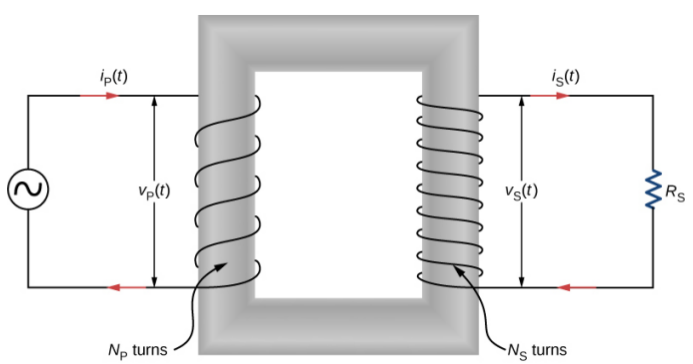
\includegraphics[width=0.45\textwidth]{transformer.png}
\caption{\label{fig:trans} The basic diagram for a \textit{transformer}...No, not Megatron the thing that gives us AC power.}
\end{figure}
In Fig. \ref{fig:trans} (left) a \textit{transformer} is depicted.  The gray square represents an iron core which ensures that the magnitude of the magnetic flux through the left solenoid \textbf{is identical to} the magnetic flux on the right solenoid.  Both solenoids are $L = 5$ cm long.  Suppose the left solenoid has $N_L = 500$ turns, and the right solenoid has $N_R = 1000$ turns.  Let the induced emf in the left solenoid be $v_L$, and the induced emf in the right solenoid be $v_R$.  Show that
\begin{equation}
\frac{v_L}{N_L} = \frac{v_R}{N_R}
\end{equation} \\ \vspace{3cm}
\item The two solenoids in Fig. \ref{fig:trans} each have volume $V = 5 \times 10^{-6}$ m$^3$, and length $l = 1.0$ cm.  What is the inductance of each, in Henries? \\ \vspace{3cm}
\item Suppose the current changes in the left solenoid of Fig. \ref{fig:trans} at a rate of 100 A s$^{-1}$.  (a) Using the inductance of the left solenoid, what is the induced emf in the left solenoid? (b) Using the result that $\frac{v_L}{N_L} = \frac{v_R}{N_R}$, calculate the induced emf in the right solenoid. \\ \vspace{4cm}
\end{enumerate}
\end{enumerate}

\end{document}